\documentclass[10pt]{article}         %% What type of document you're writing.

%%%%% Preamble

%% Packages to use

\usepackage{amsmath,amsfonts,amssymb,url}   %% AMS mathematics macros
\usepackage[numbers,sort&compress]{natbib}
\usepackage{graphicx}
\usepackage{subcaption}
\usepackage[svgnames]{xcolor}
\usepackage{listings}
\usepackage{placeins}
\usepackage{afterpage}

\graphicspath{ {./images/} }
%% Title Information.

%\textsc{\newenvironment{changemargin}[2]{%
%\begin{list}{}{%
%\setlength{\topsep}{0pt}%
%\setlength{\leftmargin}{#1}%
%\setlength{\rightmargin}{#2}%
%\setlength{\listparindent}{\parindent}%
%\setlength{\itemindent}{\parindent}%
%\setlength{\parsep}{\parskip}%
%}%
%\item[]}{\end{list}}}

\lstset{language=R,
    basicstyle=\small\ttfamily,
    stringstyle=\color{DarkGreen},
    otherkeywords={0,1,2,3,4,5,6,7,8,9},
    morekeywords={TRUE,FALSE},
    deletekeywords={data,frame,length,as,character},
    keywordstyle=\color{blue},
    commentstyle=\color{DarkGreen},
}

\title{Analysis of virulence dependence on age at infection}
\author{Petr Kouba}
%% \date{1 July 2004}           %% By default, LaTeX uses the current date

%%%%% The Document

\begin{document}
\maketitle

This document summarizes what I have learned from the structuring with respect to age at infection and its effect on virulence.
\newpage
\section{Fitting the deathrates to survival data}

I have used the same approach as before to estimate the deathrates. With the difference, that I have only considered the years \textbf{after exposure} for fitting (Notice the shift of the beggining of the age agis in plots in Figure~\ref{fig:survival_ages_5_15_30}. This time, I did the fitting for 6 groups of individuals: Those who got infected at age 5, 15 and 30 and those who were exposed, but did not get infected at age 5, 15 and 30. I used the latter three classes to estimate the natural deathrate for the former 3 groups.
\newline\newline
\textcolor{blue}{TODO: Estimate the natural deathrate from the control group and use it for all three compartments. See how much it differs.}
\newline\newline
In the following, I present the plots of the survival data and the models of the survival given our various fits for delta.

\begin{figure}[!h]
\begin{subfigure}[b]{0.6\textwidth}
    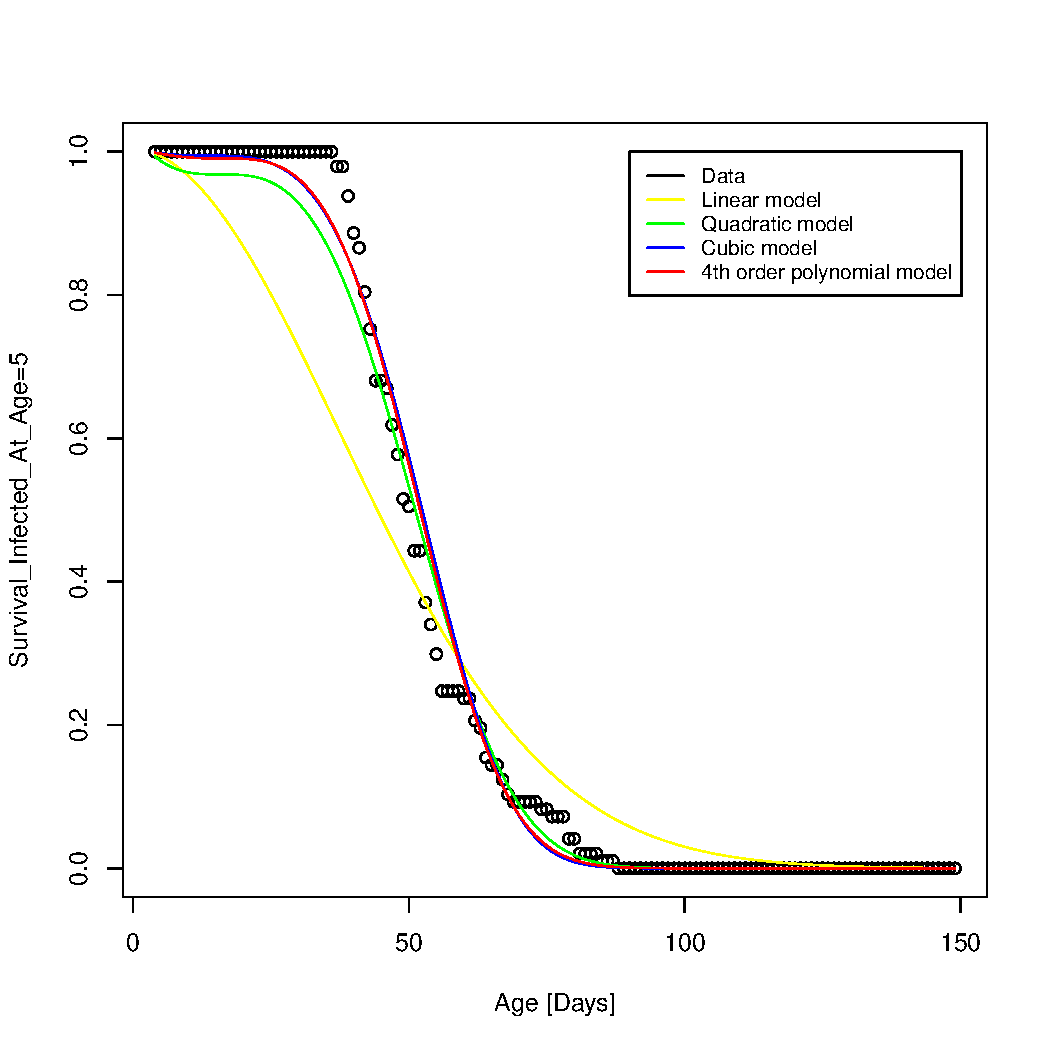
\includegraphics[width=\textwidth]{Fitting_delta_inf_at_age_5.pdf}
    \caption{Infected, age=5}
    \label{fig:subfigure_1}
  \end{subfigure}
  %
  \begin{subfigure}[b]{0.6\textwidth}
    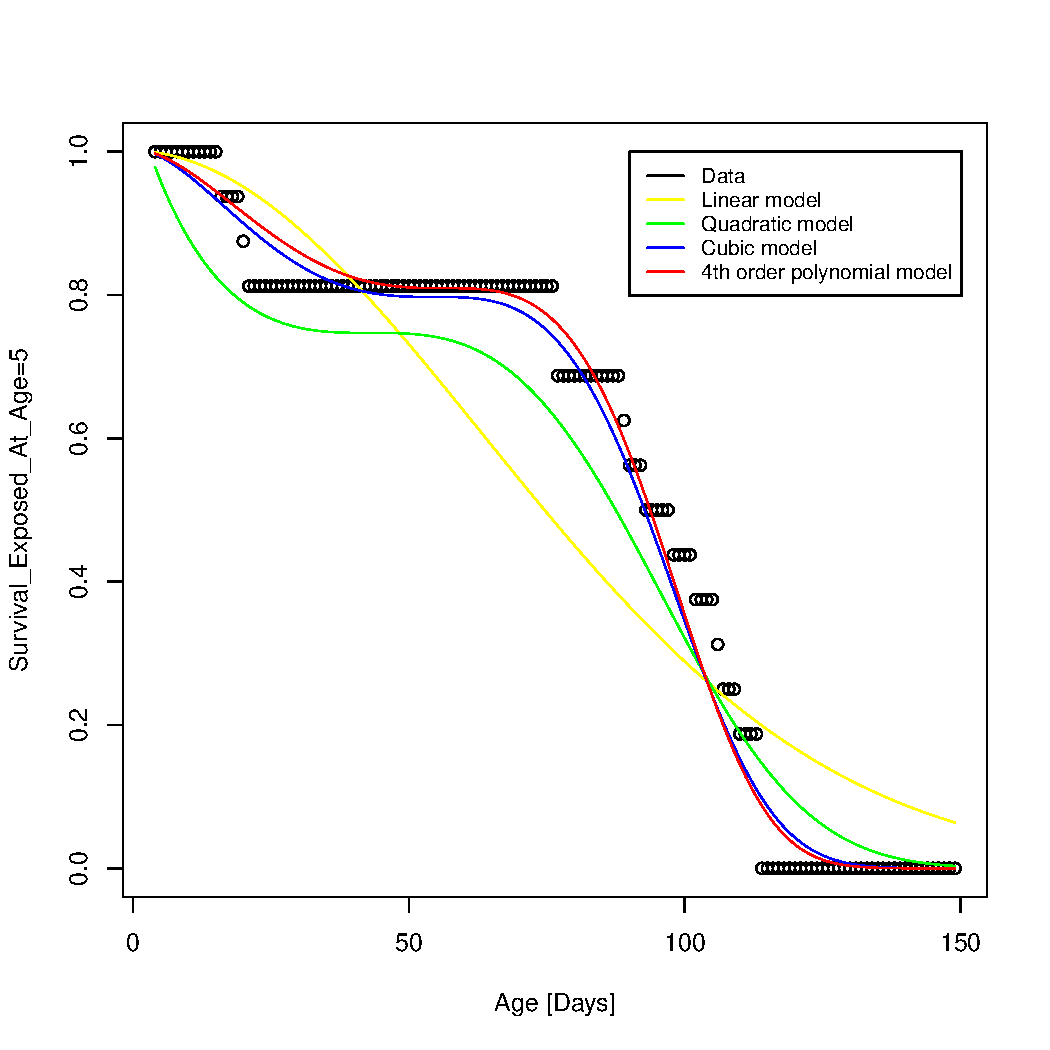
\includegraphics[width=\textwidth]{Fitting_delta_exp_at_age_5.pdf}
    \caption{Exposed but uninfected, age=5}
    \label{fig:subfigure_2}
  \end{subfigure}
\end{figure}

\begin{figure}[!ht]
\ContinuedFloat
  \begin{subfigure}[b]{0.6\textwidth}
    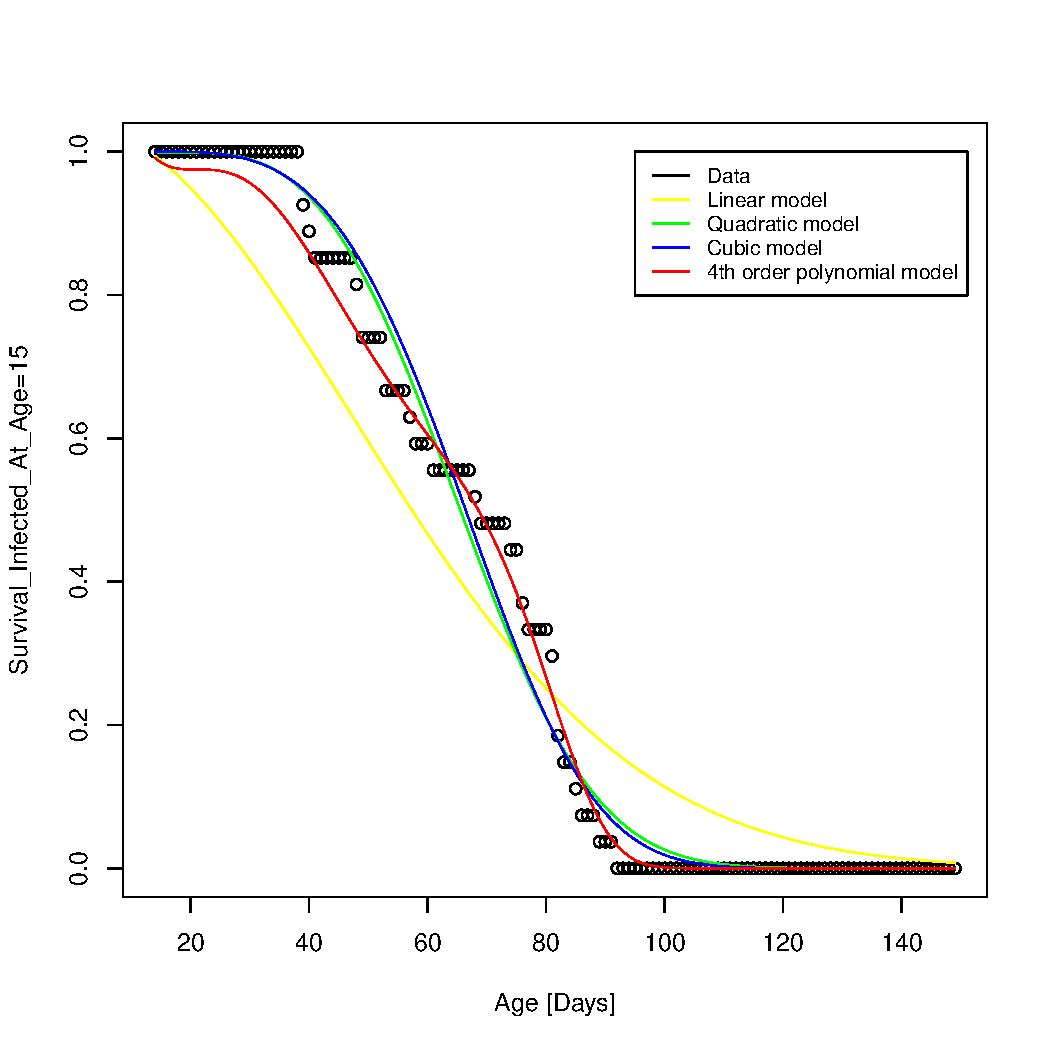
\includegraphics[width=\textwidth]{Fitting_delta_inf_at_age_15.pdf}
    \caption{Infected, age=15}
    \label{fig:subfigure_3}
  \end{subfigure}
  %
  \begin{subfigure}[b]{0.6\textwidth}
    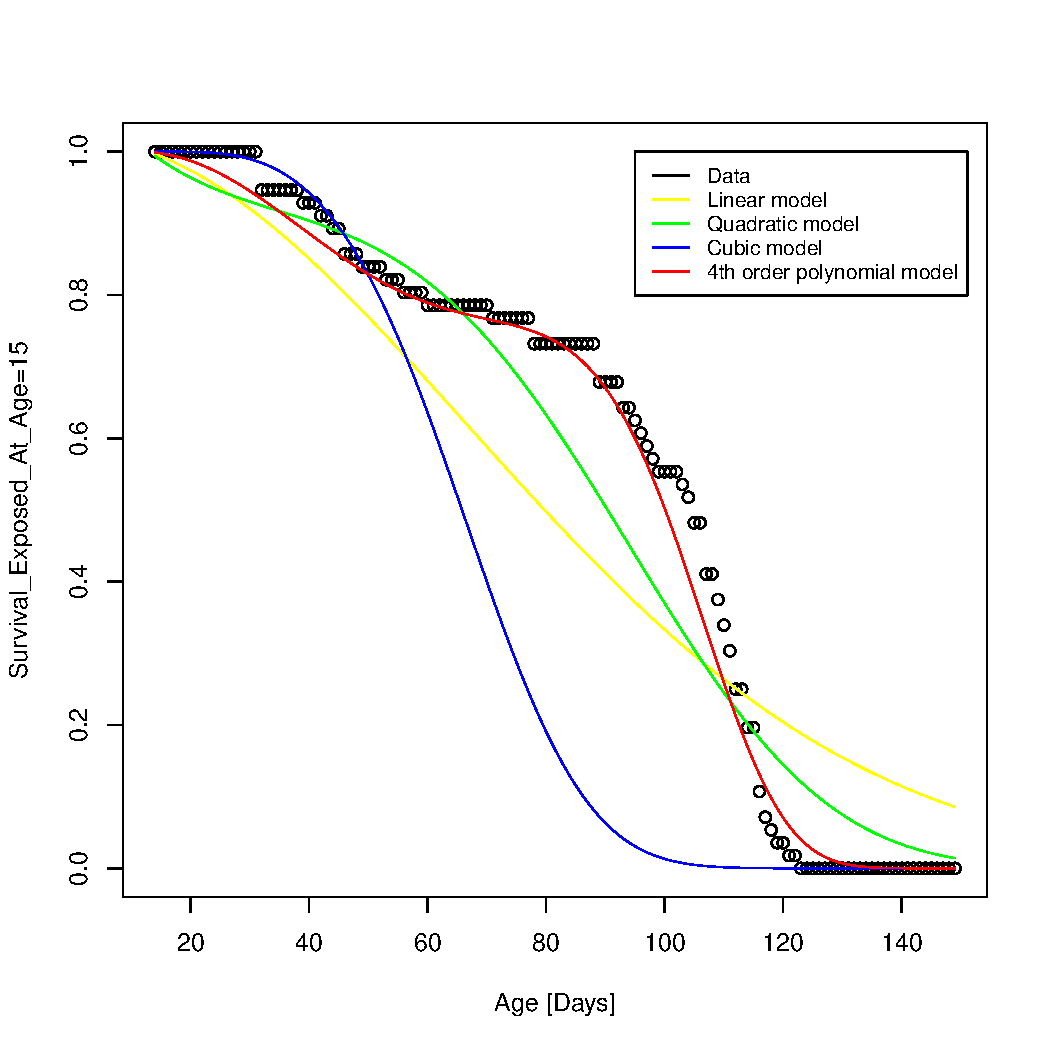
\includegraphics[width=\textwidth]{Fitting_delta_exp_at_age_15.pdf}
    \caption{Exposed, age 15}
    \label{fig:subfigure_4}
  \end{subfigure}

\begin{subfigure}[b]{0.6\textwidth}
    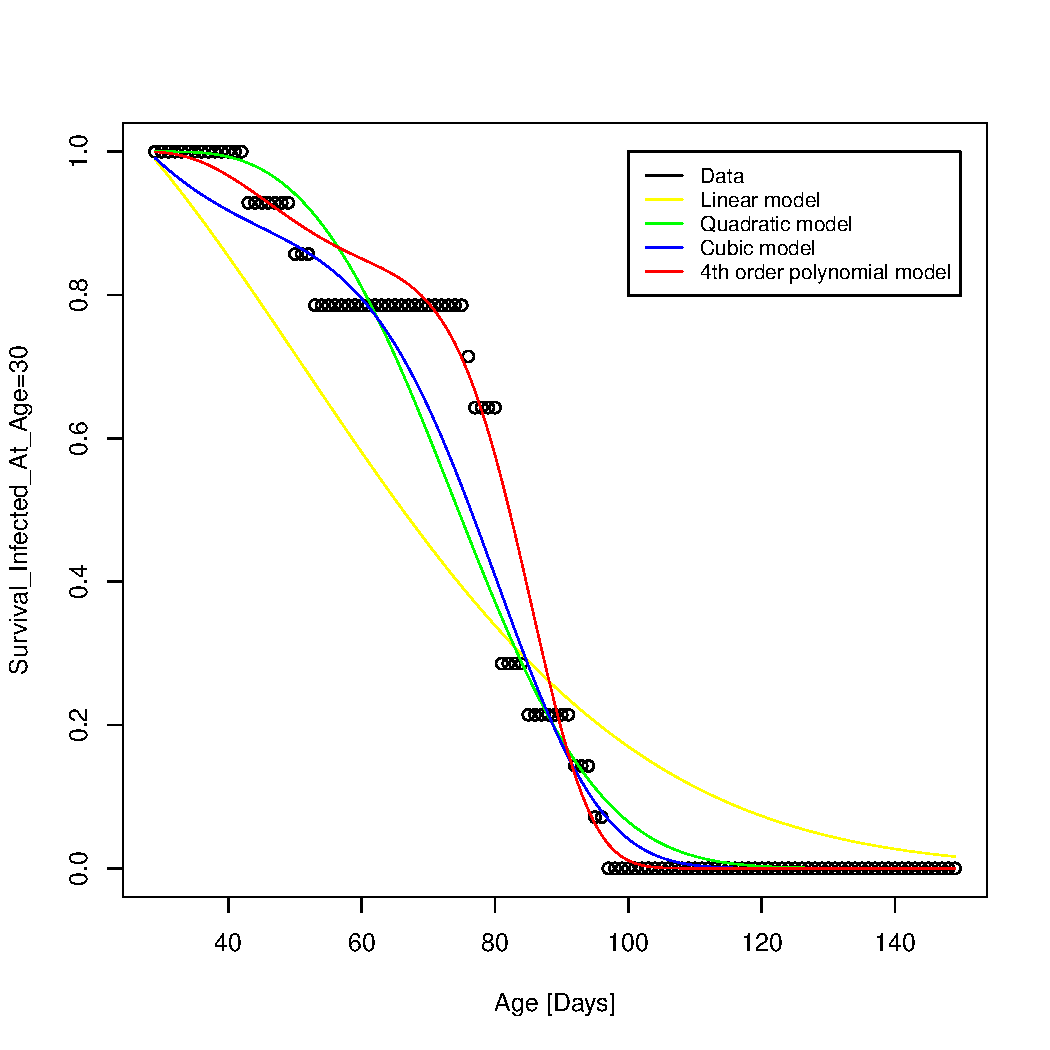
\includegraphics[width=\textwidth]{Fitting_delta_inf_at_age_30.pdf}
    \caption{Infected, age 30}
    \label{fig:subfigure_5}
  \end{subfigure}
  %
  \begin{subfigure}[b]{0.6\textwidth}
    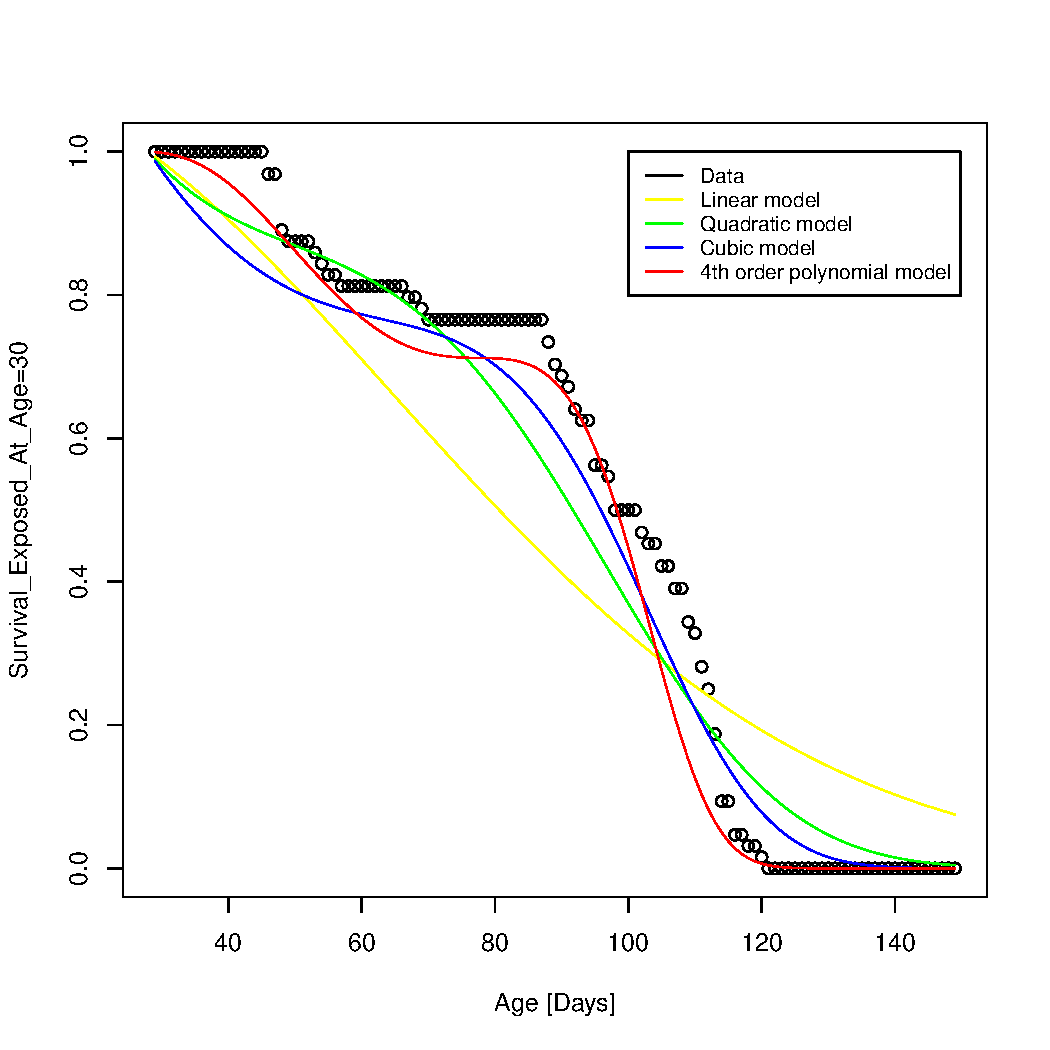
\includegraphics[width=\textwidth]{Fitting_delta_exp_at_age_30.pdf}
    \caption{Exposed, age 30}
    \label{fig:subfigure_6}
  \end{subfigure}  
  
\caption{Comparison of the survival patterns and corresponding models of survival based on different fits for delta}
	\label{fig:survival_ages_5_15_30}
\end{figure}

\clearpage
\section{Obtained virulances}

\textcolor{blue}{TODO: Death rate plots comparing the deathrates of different exposed compartments and the control population can also be put in this section}
\subsection{Choosing the best fit for each compartment}

\textcolor{blue}{TODO: I will do the likelihood ratio tests for each fit of compartment to which I fitted the delta, but first I need to get the absolute values of the likelihood including the binomial coefficients}


\textcolor{red}{Question: Supposed I have the LRTs for all the fits, but they yield polynomials of different orders as the best fits for different age-at-infection groups. Is it then legitimate to use the best fit for each compartment? Or should we stick with consistency, in that sense that we claim te order of the polynomial to be the same within a group of the same infection status (infected/exposed)?}

Sofar I used our previous results, obtained from the fitting of the total control/exposed/infected populations (before structuring wrt. age at infection) and I picked the quadratic fit for the infected individuals and $4^{th}$ order polynomial for the exposed individuals.


\subsection{Virulence with respect to the age of infection}

I have expressed the virulences for given age-of-infection groups as the difference of the death rates of infected and exposed populations:
\begin{equation}
V_{i}(a) = \delta_{i}^{infected}(a) - \delta_{i}^{exposed}(a)
\label{eq:virulence}
\end{equation}
Where $V$ stands for virulence, $a$ for age, $\delta$ for death rate and $i\in \{5,15,30\}$ is the age at infection.\newline

Taking these virulences, I have transformed them into functions of the age of infection, by shifting the independent variable (formerly age) by the age at infection $a \rightarrow (a_{infection} = a - i)$. The transformer virulences (i.e. virulences as a function of the age of infection) are plotted in the Figure~\ref{fig:virulence}.

\begin{figure}[ht!]
    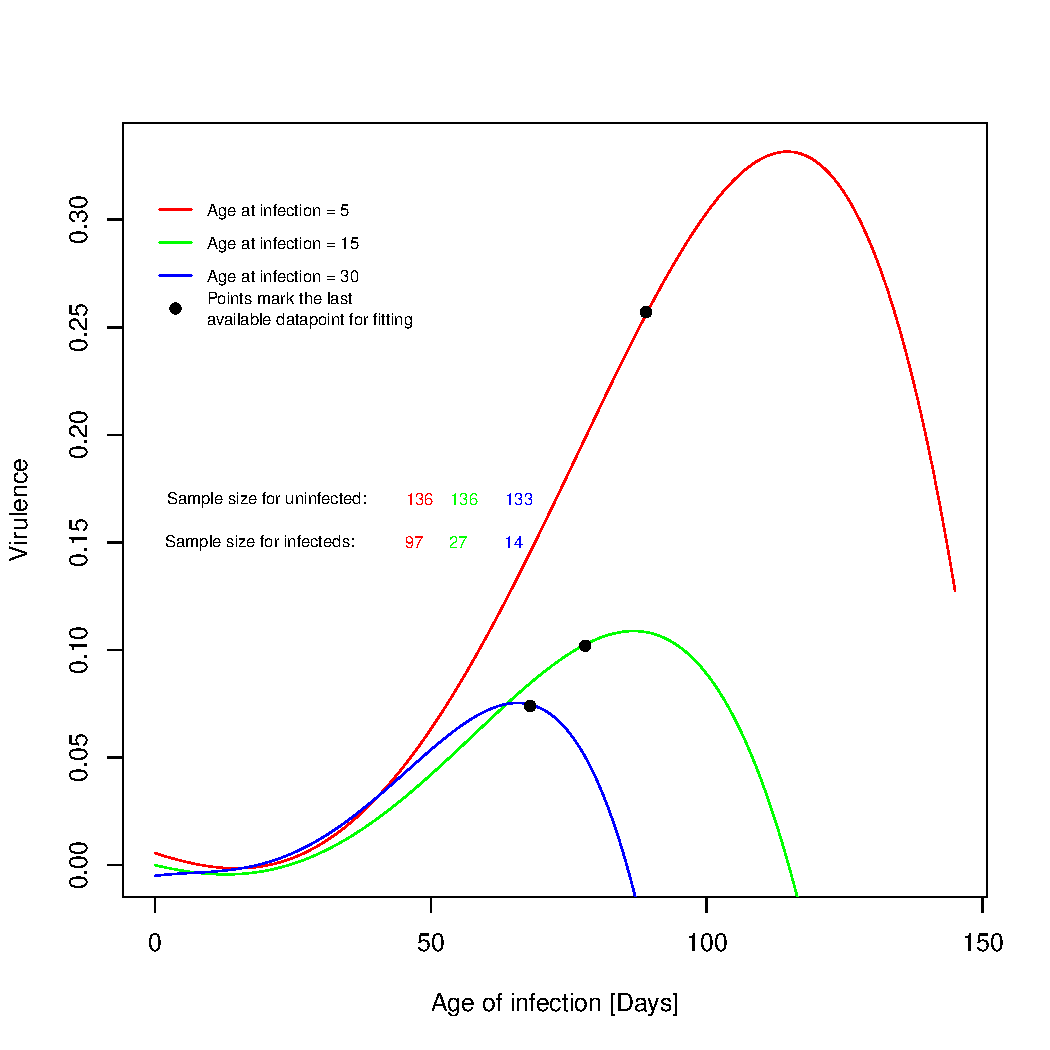
\includegraphics[width=\textwidth]{Virulences_age_of_infection_structured_same_model_for_same_infection_status.pdf}
    \caption{Virulences as functions of the age of infection, for different ages at infection. The fits might not be reliable beyond the black dots, since the dots mark the highest age of infection, where there was a datapoint serving as a support for our fit.}
\label{fig:virulence}
\end{figure}

From Figure~\ref{fig:virulence}, we can see that the virulence tends to be higher in the individuals who were infected at younger age. We now need to verify this conjecture.
\FloatBarrier
\subsection{Veryfing the significance of the influence of the age at infection on virulence}

In order to try to verify the significance of the effect of the age at infection, I came up with the following method, which seems reasonable, but I am not yet sure if it does not cause too big error amplification. We could plot the distribution of deaths due to virulence along the age of infection, for different age-at-infection classes. And our null hypothesis would be that the distribution does not depend on age at infection and therefore it should be the same for all of the 3 age-at-infection classes.
\newline\newline
Lets have a look at it step by step. First, we provide the plots of the distribution of deaths along the age of infection axis. To see the normalized histograms representing the distributions of deaths, have a look at Figure~\ref{fig:death_distributions}.

\begin{figure}[ht!]
    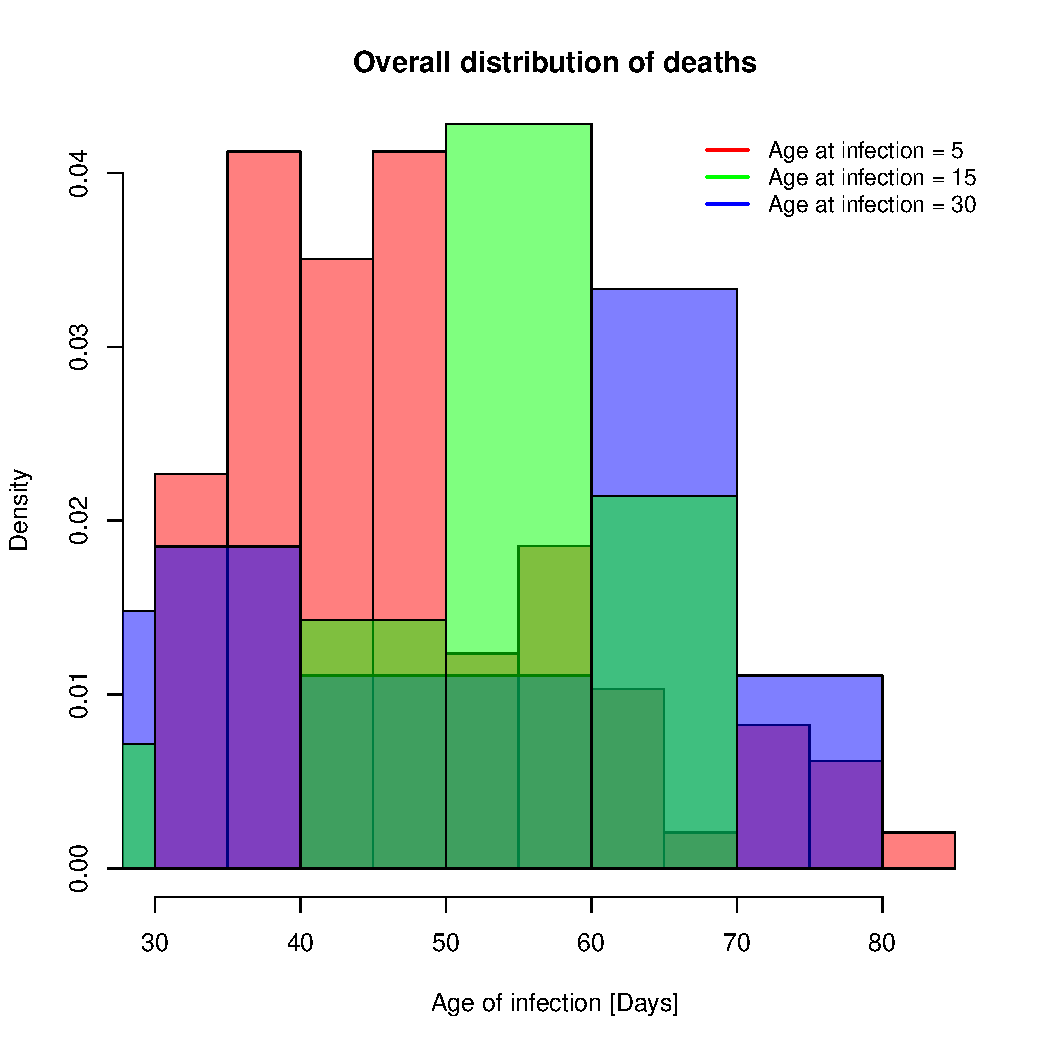
\includegraphics[width=\textwidth]{Overall_distribution_of_deaths.pdf}
    \caption{The overall distribution of deaths, for different age-at-infection classes}
\label{fig:death_distributions}
\end{figure}
\FloatBarrier

However these distribution contain lot of signal from the deaths due to natural causes. To suppress this, I decided to weight the contribution of each death to the histogram, by the ratio of virulence to the total deathrate for a given age.

For example: if an individual, infected at age 15, dies at age of infection 50 (that is at age 65), and the virulence at age 65 is 0.038, whereas the total deathrate at age 65 is 0.041, we will count it towards our histogram with the weight $0.038/0.041= 0.93$.

Weighting our histograms as described above yields the histograms provided in Figure~\ref{fig:deaths_due_virulence_distributions}

\begin{figure}[ht!]
    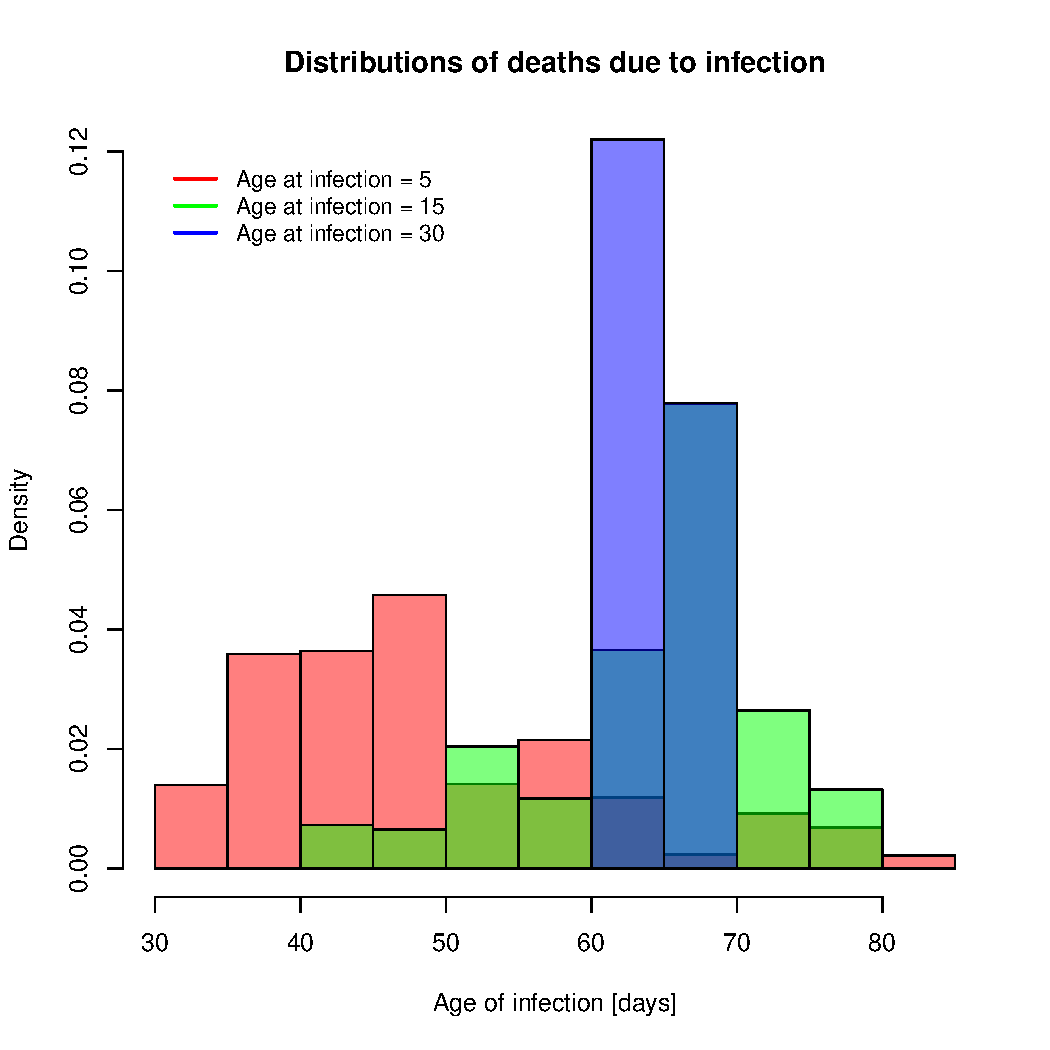
\includegraphics[width=\textwidth]{Distribution_of_deaths_due_to_virulence.pdf}
    \caption{The distribution of deaths due to virulence only, for different age-at-infection classes}
\label{fig:deaths_due_virulence_distributions}
\end{figure}
\newpage
For some ages, there was a negative virulence, which does not make any sense and it is only an imperfection, which can be understood from the equation~\ref{eq:virulence}. It simply happened that for some ages, we had higher death rate in the exposed population then in the infected population. We explain this by being in the stage of the infection when it does not kill the host and due to some fluctuations we even had a higher death rate in the exposed population. Therefore, we interpret the virulence in those years to be 0, this fixed our problem with potentially negative weights in the histogram.

From the Figure~\ref{fig:deaths_due_virulence_distributions} we can once again see, that the hosts who were infected at younger age tend to die at earlier age than the hosts who got infected later, which again supports the conjecture that the infection is more virulent in younger hosts.

I think by the above procedure I have transformed the problem into a more suitable form, since this now seem better fit for hypothesis testing. I pick a suitable distribution and test the probability that all of those three distributions in Figure~\ref{fig:deaths_due_virulence_distributions} were distributed according to it.

\textcolor{blue}{TODO: Think about how to choose the distribution for our null hypotheses. Perform the hypothesis testing, to potentially rule out the hypothesis that virulence is independent of the age at infection.}


\bibliographystyle{unsrtnat}
\bibliography{bibliography_SIE_model}

\end{document}


